\chapter{Introduction}\label{Ch:Intro}
When we open the history book of the universe, we find blank pages in the middle. These blank pages correspond to periods in cosmic history where we have no direct data. One such time period is the $''$Dark Ages$''$ ($z \sim 1100$ to $z \sim 30$), which started when light and matter decoupled during recombination and ended with the births of the first stars in the universe. Following that came the $''$Cosmic Dawn$''$ ($z\sim 30$ to $z\sim 10$), when the first stars lived, died and impacted the universe around them. Very little is known about these times; as no one has been able to observe them directly. 

Recently, the development of \cm cosmology has provided a potential tool for measuring these eras of our history and filling in some of the blanks. There are a number of experiments that seek to utilize this tool to study the universe. Many of the experiments are interested in the Dark Ages, Cosmic Dawn, or the Epoch of Reionization that immediately follows them.  

\section{Hydrogen \cm Signal}
In order to discuss \cm cosmology, we first need to understand the basic physics behind the signals that we are studying. There are four components that need to be defined to facilitate this understanding. First, we need to review the atomic states of hydrogen and in particular the hyperfine splitting of the ground state. Second, we need to define the spin temperature of a cloud of neutral hydrogen atoms and discuss how emission and absorption change the spin temperature. Third, we need to define brightness temperature and detail how that temperature can change when it passes through a cloud of hydrogen gas. Fourth, we need to combine spin temperature and brightness temperature via the opacity of a cloud of hydrogen gas. 

\subsection{Hydrogen Atomic States}
To understand the \cm signal, we start with the structure of the hydrogen atom; one proton and one electron. The proton and electron each have a spin $\pm \frac{1}{2}$, which leads to a splitting of the ground state of hydrogen depending on the total spin angular momentum of the atom. The energy of the atom is lower when the spins are anti-aligned and the total spin angular momentum of the atom is zero than when the spins are aligned with a total spin angular momentum of one. This energy difference is called $''$hyperfine$''$ splitting; with the spin 0 state being a singlet and the spin 1 state being a triplet (and therefore three times more likely). The energy difference from this splitting is $h \nu_{10}$, where $\nu_{10}=1420.405$ MHz and $\lambda_{10} =  21$ centimeters.  

\subsection{Spin Temperature}
When working with a cloud of hydrogen atoms rather than a single atom, we need to compare the number of atoms in the two states within the cloud. To do this, we define the spin temperature using Boltzmann's law for a cloud in thermodynamic equilibrium. A spin temperature (\ts) is defined with the ratio of the the two states $n_1/n_0$. 

\begin{equation}\label{Eq:T_s}
\frac{n_1}{n_0} \equiv 3 e^{- h \nu_{10} / kT_S} = 3 e^{-T_*/T_S}
\end{equation} 

\subsection{Emission and Absorption} \label{Sec:dT_S}
Change of the spin temperature occurs through emission and absorption of \cm photons corresponding to a transition between the two spin states. Transitions occur when the atom either spontaneously emits a photon or is induced to emit or absorb a photon due to external forces. These transitions can be described using a differential equation (Equation \ref{Eq:dn}), and each type of transition (m) has a different $X^m_{ij}$. If the cloud is in equilibrium, the rates of change are related by $d n_0/dt = - d n_1 /dt$, so that $n_0 \sum^m X^m_{01} = n_1 \sum^m X^m_{10}$ at all times. 

\begin{equation} \label{Eq:dn}
\big( \frac{d n_i}{dt} \big)_m = X^m_{ij} n_i
\end{equation}

Spontaneous emission due to a transition between the spin states is extremely rare, as the triplet state has a lifetime of over 10 million years. The exact rate is set by the Einstein A coefficient ($A_{10}$), which is defined as: 

\begin{equation}
A_{10} = \frac{64 \pi^4 \beta^2}{3 h \lambda^3} = 2.85 x 10^{-15} sec^{-1}
\end{equation}

where $\beta$ is the Bohr magneton. On the other hand, absorption and induced emission can be caused by a number of different mechanisms. 

The first is incident radiation from an external source such as Cosmic Microwave Background (CMB) photons. The coefficients for this source are $X^R_{01} = B_{01} I_\nu$ and $X^R_{10} = B_{10} I_\nu $, with $B_{01} = 3 B_{10}$ and $B_{10} I_{\nu} = A_{10} \lambda^2 I_\nu / 2 h \nu_{10}$. 

%Incident radiation gives coefficients $X^R_{01}$ such that $I_\nu B_{01} = 3 A_{10} \lambda^2 I_\nu/2 h \nu_{10}$ and $B_{01}/B_{10} = 3 e^{-T_*/T_R}$.  

In addition to incident radiation of wavelength \cm, there are two other sources of change for $n_0$ and $n_1$. The first is collisions between atoms and electrons in the gas cloud, which has coefficients $C_{01}$ and $C_{10}$. Because the system is in thermodynamic equilibrium, we can define a kinetic temperature (\tk) using the transition coefficients $C_{01}/C_{10} \equiv 3 e^{-T_*/T_K}$. 

The second source of change is light at other wavelengths causing changes to the atoms. This second impact is known as the Wouthuysen-Field mechanism \cite{wouthuysen_1952}\cite{field_1958} and will be discussed in greater detail in Section \ref{Sec:WFM}. For now, we'll just define a light temperature ($T_L$) using the same form as the other temperatures ($L_{01}/L_{10} = 3 e^{-T_*/T_L}$).

When we combine all of these sources of transitions, we get the following equation: 

\begin{equation}
n_1(A_{10} + B_{10} I_\nu + C_{10} + L_{10}) = n_0 (B_{01} I_\nu + C_{01} + L_{01})
\end{equation}

Rearranging, we get an equation for $n_1 / n_0$ and the spin temperature:

\begin{equation}
\frac{n_1}{n_0} = 3 e^{-T_*/T_S} = \frac{B_{01} I_\nu + C_{01}+ L_{01}}{A_{10}+ B_{10} I_\nu + C_{10} +L_{10}}
\end{equation}

To simplify this equation we use the fact that $T_* = 68.1 mK$ and $T_S \gg T_*$ to approximate the exponentials ($e^{-T_*/T} \simeq 1-T_*/T$) and rearrange to get:

\begin{equation}\label{Eq:dT_s}
T_s = \frac{T_{R} + x_K T_{K} + x_{L} T_{L}}{1+x_K +x_{L}}
\end{equation}

where the coupling coefficients are $x_K = T_* C_{10}/A_{10} T_K$ and $x_L = T_* L_{10} / A_{10} T_L$, and $T_R$ is the incident radiation temperature. 

\subsection{Brightness Temperature}
The primary sources of incident radiation for hydrogen gas clouds are blackbody sources such as the CMB.  These blackbody sources have an energy distribution ($B_\nu (T)$) defined by the Planck spectrum:

\begin{equation}
I_{\nu} = B_{\nu}(T) = \frac{ 2 h \nu^3 / c^2}{e^{h \nu / k T}-1}
\end{equation}

For long wavelengths like the ones we are considering, we can use the Rayleigh-Jeans approximation ($B_{\nu} (T) \simeq (2 k \nu^2 / c^2) T$) to give us the brightness temperature ($T_b (\nu)$) \cite{carroll2007}. 

This brightness temperature will change as the light travels through the universe. There are two components of this change, signal evolution due to the expansion of the universe and signal evolution due to the light passing through gas clouds. Expansion of the universe causes a signal decrease from its original strength. The decrease is $\propto 1/(1+z)$. 

When the light passes through a gas cloud, the rate at which the brightness temperature changes can be written in terms of the opacity of the cloud (\tu). The brightness temperature after passing through the cloud can be written as:

\begin{equation}
T_b (\nu) = T_{C} (\nu) (1-e^{-\tau_\nu}) +T_{R} e^{-\tau_\nu}
\end{equation}

where $T_{C}$ is the cloud temperature and $T_{R}$ is the original brightness temperature when it enters the cloud. As observers, what we actually care about and can observe is $\delta T_b (\nu) = T_b (\nu) - T_R  (\nu)$. 

\subsection{Opacity ($\tau_\nu$)}
So, in order to measure the change in brightness temperature caused by passing through a cloud of gas, we need to know the cloud's opacity at a given frequency. The opacity (\tu) is defined as an integral along a line of sight throught the cloud of the absorption rate of photons at the frequency $\nu$. In this case, what we care about is $\tau_{21-cm}$, which has a defined opacity:

\begin{equation}
\tau_{\nu} = \frac{3 c^2 A_{10}}{8 \pi \nu^2 } (1-e^{-T_*/T_S}) \int ds \phi (\nu) n_0(s)
\end{equation}

where $\phi (\nu)$ is the line profile of the hydrogen \cm spectral line at each position such that $\int \phi(\nu) d \nu = 1$ at that position and $n_0 (s)$ is the number of hydrogen atoms at each position that are in the spin 0 state. A detailed formulation for \tu depends on the details of the hydrogen gas cloud, as will be discussed in Section \ref{Sec:IGM}. 


\section{The Intergalactic Medium (IGM)}\label{Sec:IGM}
Using the physics discussed in the previous section, we can study the intergalactic medium (IGM) as a hydrogen gas cloud that changes the brightness temperature of photons from the Cosmic Microwave Background (CMB) as they pass through the cloud. The modified brightness temperature ($\delta T_b (\nu)$) has a spectrum in frequency and space that depends on the history of the IGM. In order to make a prediction of this spectrum, we need to have a model of the history of the IGM during the time periods that we want to study. This model will allow us to calculate a predicted \ts and \tu in the IGM throughout its history. 

\subsection{IGM Fundamentals}
\subsubsection{Opacity ($\tau_\nu$)}
To calculate the opacity of the IGM requires a model of atomic density. In this model there are a few significant terms that all combine to give a column density of neutral hydrogen ($N_{HI}$) through the IGM. This column density is $N_{HI}/4 = \int ds n_0 (s)$, where the factor of 4 comes from the sum of states (triplet plus singlet). The column density can also be written as the fraction of hydrogen that is neutral ($x_{HI}$) times the number of hydrogen atoms along the line of sight ($n_H (z)$) times the line of sight ($s$). With all of these factors, we can re-write the opacity as:

\begin{equation}
\tau_{\nu} \approx 0.0092 (1+\delta) (1+z)^{3/2} \frac{x_{HI}}{T_S} \big[ \frac{H(z)/(1+z)}{dv_{\parallel}/dr_{\parallel}} \big]
\end{equation} 

where $(1+\delta)$ is the matter density at a given position, $dv_{\parallel}/dr_{parallel}$ is the gradient of proper velocity along the line of sight, and $H(z)$ is the Hubble constant. 

\subsubsection{Brightness Temperature Change ($\delta T_b$)}
Because the opacity is $\propto T^{-1}_S$, for small $T_S$ we can use the taylor expansion $e^{-\tau_\nu} \approx 1-\tau_\nu$. This allows us to write the change in brightness temperature of CMB photons due to passing through the IGM as:

\begin{equation}\label{Eq:dT_b}
\delta T_b = \frac{T_S - T_\gamma}{1+z}(1-e^{-\tau_\nu}) \approx 9 (1+\delta) (1+z)^{1/2} (1-\frac{T_\gamma}{T_S})x_{HI} \big[ \frac{H(z)/(1+z)}{dv_{\parallel}/dr_{\parallel}} \big] mK
\end{equation}

where $T_\gamma$ is the CMB photon temperature, which also acts as the incident radiation temperature ($T_R$) in Equation \ref{Eq:dT_s}. 

\subsubsection{Wouthuysen-Field Mechanism}\label{Sec:WFM}
Given that the spin temperature of the IGM is a significant term in the brightness temperature equation, we need to understand how it can vary over time. As discussed in Section \ref{Sec:dT_S}, the spin temperature of hydrogen in the IGM is coupled to three sources during its history. The first source is the CMB (\tg), which provides a source of external radiation ($T_R$). The second source is the kinetic temperature of the gas (\tk), which characterizes the thermal motion of the atoms in the gas. The third and final source is external photons corresponding to the transitions between states of the hydrogen atom besides the \cm transition ($T_L$), particularly the \lya transition. 

The mechanism for the coupling between the hydrogen spin state and \lya photons is called the Wouthuysen-Field Effect \cite{wouthuysen_1952}\cite{field_1958} and can be understood by going back again to the atomic states of the hydrogen atom. Just as we've discussed for the \cm transition, external photons with an energy corresponding to the \lya wavelength ($\lambda = 121.6$ nm) can induce a transition from the ground state of hydrogen (1S) to its first excited state (2P). However, conservation of total spin angular momentum for the hydrogen atom sets the selection rules for spontaneous emission due to transitions back to the ground state. 

There are two pathways set by the selection rules for the hydrgoen to spontaneously emit \lya photons. If the original 1S state is the singlet spin zero state $_0S_{1/2}$, then it will transition to the $_1P_{3/2}$ state and then back to the triplet spin one state $_1S_{1/2}$. On the other hand, if the original 1S state is the triplet spin one state $_1S_{1/2}$, then it will transition to the $_1P_{1/2}$ state and then back to the singlet spin zero state $_0S_{1/2}$. This process redistributes the the neutral hydrogen atoms in the ground state such that $n_tot = n_0 + n_1$ is unchanged, but the spin temperature is changed. 

The exact magnitude of the change will depend on the distribution of photons around the \lya line, since the frequency of the photon needed for each of the two transitions is slightly different. This can be written in terms of the two components we identified previously, the coupling term $x_{L} = x_{Ly-\alpha}$ and the light temperature $T_L = T_{Ly-\alpha}$. 

The distribution of \lya photons is set by collisions within the IGM, and approximates a blackbody curve with temperature $T_{Ly-\alpha} = T_K$. Meanwhile, the \lya coupling term is proportional to the intensity of \lya photons produced by external sources of light such as stars. 

\subsection{History of the IGM}
In the early universe before galaxies came into existence, the entire universe was filled with a medium that is the progenitor of the IGM. From the Cosmic Microwave Background, we know that at $z \sim 1100$ the IGM was a nearly homogeneous gas of protons, free electrons, and atoms; most of which were neutral hydrogen atoms. Within the gas were small inhomogeneities in the matter density that would eventually grow into galaxies, but the overall gas density was high enough that collisions between baryons were common throughout the gas. 

\begin{figure}[htb]
\begin{center}
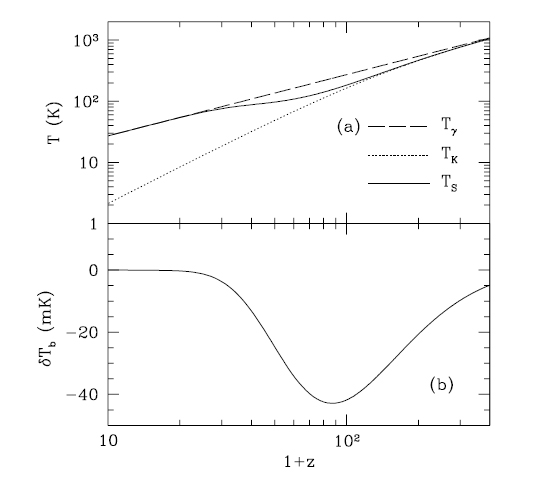
\includegraphics[width=0.95\linewidth]{Introduction/figures/dark_ages_global_spectrum.jpg}
\caption{(a) Plot of $T_S$, $T_\gamma$, and $T_K$ during the dark ages and (b) $\delta T_b$ during the same period given only collisional coupling from furlanetto et. al. \cite{furlanetto_2006}}
\label{Fig:da_global}
\end{center}
\end{figure}

\subsubsection{Dark Ages}
During the dark ages, the universe expanded at a rate defined by the Hubble parameter. Initially, the IGM was dense enough for Compton scattering between CMB photons and free electrons in the IGM to set \tk$=$\tg. But as the gas adiabatically expanded, thermal decoupling caused \tk to decrease. At this time, collisions between baryons in the IGM kept $x_K$ large, so that the spin temperature decreased below the CMB temperature. 

However, this coupling gradually decreased as the rate of collisions between baryons decreased, and the spin temperature increased back to match the CMB temperature. The process of cooling and decoupling created a dip in \ts, which most models predict should be centered around $z \sim 80 $ \cite{furlanetto_2006}. Figure \ref{Fig:da_global} shows one model prediction for the relevant temperatures including $T_\gamma$, $T_K$, $T_S$ and $\delta T_b$ before star formation. 

At the same time, the first generation of stars began to form in the overdense regions of space. 

\textcolor{blue}{Need to add discussion of first stars.}

\begin{figure}[htb]
\begin{center}
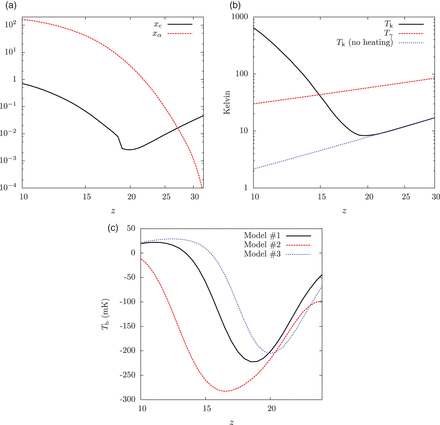
\includegraphics[width=0.95\linewidth]{Introduction/figures/ts_evolution.png}
\caption{Plots of (a) $x_K$ and $x_{Ly-\alpha}$, (b) $T_\gamma$ and $T_K$ with or without x-ray heating, and (c) $\delta T_b$ during the Cosmic Dawn for different models of star formation from natarajan et. al. \cite{natarajan_2014}}
\label{Fig:cd_global}
\end{center}
\end{figure}

\subsubsection{Cosmic Dawn}
With the birth of the first stars, light began to propogate through the IGM. This light included \lya photons, which re-coupled \ts and \tk via the Wouthuysen-Field mechanism. Since the kinetic temperature of the IGM was at this point much lower than \tg, this re-coupling decreased \ts. 

Meanwhile, x-ray photons were produced by two types of sources among the first Pop.III stars. One source was electrons accelerated by supernovae to relativistic speeds. When these electrons undergo inverse Compton scattering, x-ray photons are produced. The other source was high-mass x-ray binary stars, which occur when massive stars on the main sequence lose material through accretion onto a compact neighbor such as a neutron star, black hole or white dwarf star. 

These high energy photons heated the IGM through a combination of photoionization of Hydrogen or Helium and collisions with IGM components \cite{furlanetto_2006}. 

Depending on the rate of x-ray heating compared to the rate of \lya coupling, the spin temperature is predicted to dip during the period where $x_k>0$ and \tk is less than \tg. By varying the model of first star formation, the exact shape of the dip in the spin temperature can be adjusted. Most models predict a dip centered around $z\sim20$, with a width of $0 \leq z \leq 10$ and a depth of $0\leq \Delta T \leq 300 mK$. Figure \ref{Fig:cd_global} shows a few models of global $\delta T_b$  during the Cosmic Dawn, as well as some of the parameters that feed into the brightness temperature variance. 

\textcolor{red}{Add figure here to show reionization.}

\subsubsection{Epoch of Reionization}
As the kinetic temperature of the gas continued to rise, it reached the threshold where Equation \ref{Eq:T_s} breaks down \textcolor{red}{Why?} and the spin temperature plateaued at its maximum level. Meanwhile, the propogation of x-ray photons through the IGM also began to ionize the hydrogen atoms. Since the brightness temperature of the \cm signal is also proportional to the amount of neutral hydrogen ($x_{HI}$) present in the IGM, as shown in Equation \ref{Eq:dT_b}, this ionization process caused a gradual decrease in the average \cm signal. 

\section{Measuring the \cm Signal}

\subsection{Intensity Mapping and the \cm Power Spectrum}

\subsection{Average (Global) \cm Frequency Spectrum}

\section{\cm Experiments}

\subsection{Mapping Experiments}

\subsubsection{GBT-IM Experiment}

\subsubsection{CHIME Experiment}

\subsection{Global Experiments}

\subsubsection{SCI-HI Experiment}